\documentclass[aspectratio=169,10pt]{beamer}

\usepackage[T1]{fontenc}
\usepackage{lmodern}
\usepackage{booktabs}
\usepackage{graphicx}
\usepackage{xcolor}

\definecolor{navy}{HTML}{18344A}
\definecolor{blue}{HTML}{3274A3}
\definecolor{coral}{HTML}{C85F4A}
\definecolor{mint}{HTML}{E7F1EE}
\definecolor{warm}{HTML}{F9E9E3}
\definecolor{ink}{HTML}{202124}

\setbeamercolor{normal text}{fg=ink,bg=white}
\setbeamercolor{frametitle}{fg=navy,bg=white}
\setbeamercolor{structure}{fg=blue}
\setbeamertemplate{navigation symbols}{}
\setbeamertemplate{footline}{\hfill\color{navy}\insertframenumber\hspace{1.2em}\vspace{0.7em}}
\setbeamertemplate{itemize item}{\color{coral}\textbullet}
\setbeamertemplate{itemize subitem}{\color{blue}\textendash}
\setbeamerfont{frametitle}{series=\bfseries,size=\Large}

\newcommand{\datasetbox}[4]{%
  \begin{beamercolorbox}[wd=0.46\textwidth,sep=1.0em,rounded=false,shadow=false]{normal text}
    \colorbox{#1}{\parbox[c][0.43\textheight][c]{0.91\textwidth}{%
      \centering
      {\color{navy}\Large\bfseries #2}\par\vspace{0.75em}
      {\large #3}\par\vspace{0.8em}
      \raggedright\normalsize #4
    }}
  \end{beamercolorbox}%
}

\begin{document}

\begin{frame}
  \vspace{0.35em}
  {\color{coral}\large\bfseries PART 3: IN-CLASS EXERCISE}\par\vspace{0.35em}
  {\color{navy}\Huge\bfseries Logistic Regression vs. KNN}\par\vspace{0.35em}
  {\large Two datasets, one question}\par\vspace{1.0em}

  \begin{columns}[T,onlytextwidth]
    \column{0.49\textwidth}
    \datasetbox{mint}{Breast Cancer}{Real classification data}{569 observations\\30 features\\Malignant vs. benign}
    \column{0.49\textwidth}
    \datasetbox{warm}{\texttt{make\_moons}}{Simulated nonlinear data}{300 observations\\2 features\\Curved two-moon pattern}
  \end{columns}

  \vfill
  \begin{center}
    \parbox{0.88\textwidth}{\centering\color{navy}\Large\bfseries How do the same classifiers behave on different data structures?}
  \end{center}
\end{frame}

\begin{frame}{Your Coding Task}
  \begin{columns}[T,onlytextwidth]
    \column{0.54\textwidth}
    {\color{navy}\large\bfseries Complete five TODOs in the starter file}\par\vspace{0.55em}
    \begin{enumerate}
      \item Build Logistic Regression.
      \item Set KNN to $k=5$.
      \item Make a stratified 70/30 train-test split.
      \item Fit fresh copies of both models.
      \item Compare both datasets.
    \end{enumerate}
    \vspace{0.55em}
    \colorbox{warm}{\parbox{0.91\textwidth}{\centering\color{ink}\large You have about four minutes.}}

    \column{0.42\textwidth}
    \colorbox{mint}{\parbox[c][0.68\textheight][c]{0.84\columnwidth}{%
      \centering\color{navy}\large\bfseries Use the same workflow twice\par\vspace{1em}
      \raggedright\color{ink}\small
      \texttt{StandardScaler()}\\
      \hspace{1em}$\downarrow$\\
      \texttt{LogisticRegression(max\_iter=1000)}\\[0.7em]
      \texttt{StandardScaler()}\\
      \hspace{1em}$\downarrow$\\
      \texttt{KNeighborsClassifier(}\\
      \hspace{1em}\texttt{n\_neighbors=5)}\\[0.35em]
      \color{coral}Breast Cancer: accuracy + malignant recall\\[0.4em]
      \color{blue}\texttt{make\_moons}: accuracy + boundary shape
    }}
  \end{columns}
\end{frame}

\begin{frame}{Breast Cancer: Accuracy Is Not Enough}
  \vspace{0.35em}
  \begin{center}
    \begin{tabular}{lrr}
      \toprule
      \textbf{Model} & \textbf{Test accuracy} & \textbf{Malignant recall} \\
      \midrule
      Logistic Regression & \color{navy}\textbf{0.988} & \color{navy}\textbf{0.984} \\
      KNN ($k=5$) & 0.959 & 0.891 \\
      \bottomrule
    \end{tabular}
  \end{center}
  \vspace{0.9em}
  \begin{columns}[T,onlytextwidth]
    \column{0.47\textwidth}
    \colorbox{warm}{\parbox[c][0.27\textheight][c]{0.91\textwidth}{\centering\color{ink}\large\bfseries Discussion\\[0.55em]\normalsize Is the model with the highest accuracy always the safest model?}}
    \column{0.49\textwidth}
    \colorbox{mint}{\parbox[c][0.27\textheight][c]{0.91\textwidth}{\centering\color{ink}\large\bfseries Error cost matters\\[0.45em]\normalsize False negative: malignant $\rightarrow$ benign\\Malignant label is \texttt{0}, so use \texttt{pos\_label=0}.}}
  \end{columns}
  \vfill
  \centering\color{navy}\large\bfseries In medical classification, recall can matter as much as accuracy.
\end{frame}

\begin{frame}{\texttt{make\_moons}: Boundary Shape Matters}
  \centering
  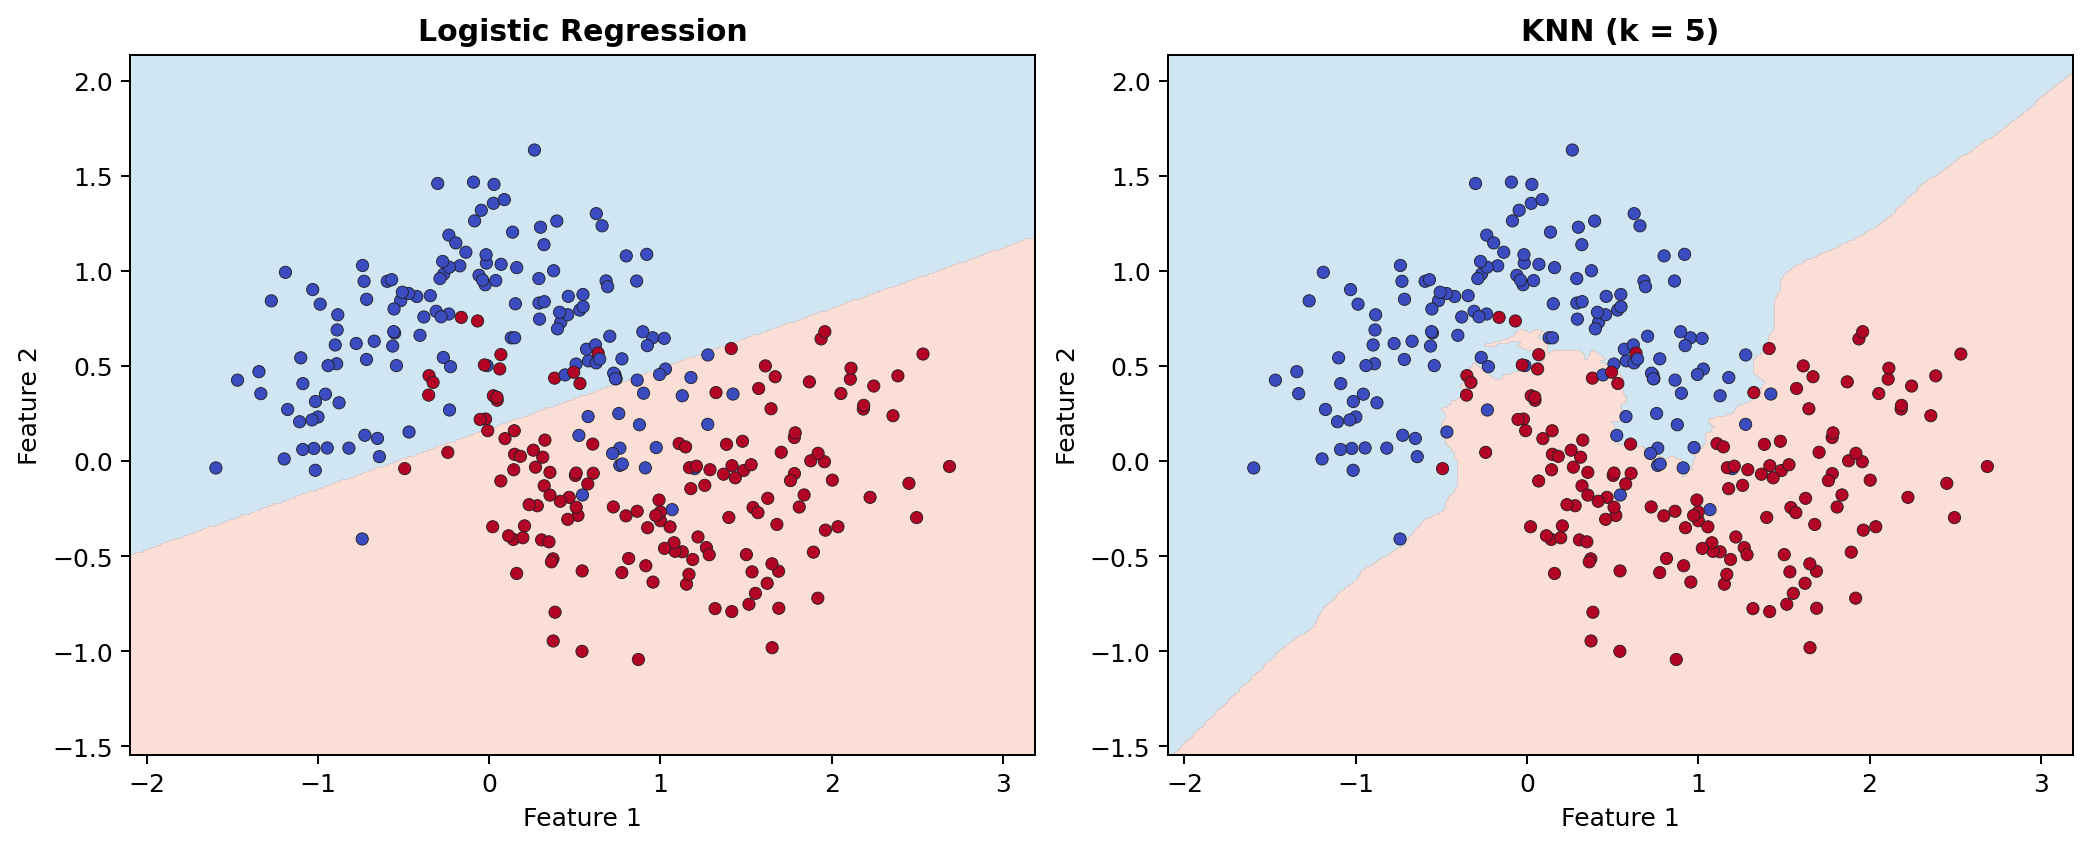
\includegraphics[width=0.94\textwidth,height=0.63\textheight,keepaspectratio]{assets/decision_boundaries.png}\par\vspace{0.25em}
  \begin{columns}[T,onlytextwidth]
    \column{0.47\textwidth}
    \centering\color{navy}\large\bfseries Logistic Regression\\[-0.1em]
    \normalsize Linear boundary: accuracy $=0.856$
    \column{0.47\textwidth}
    \centering\color{coral}\large\bfseries KNN ($k=5$)\\[-0.1em]
    \normalsize Flexible local boundary: accuracy $=0.911$
  \end{columns}
  \vfill
  \centering\color{navy}\large\bfseries Choose models using data structure, evaluation goals, and error cost.
\end{frame}

\end{document}
